\mbox{$\displaystyle -\,$\,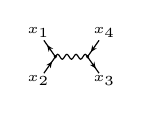
\begin{tikzpicture}[x=0.340cm, y=0.340cm, line width=0.420pt, baseline={([yshift=-0.6ex]0,0)}]
  \draw plot[smooth, tension=0.7] coordinates {(-0.600,0.000) (-0.557,0.065) (-0.514,0.093) (-0.471,0.065) (-0.429,0.000) (-0.386,-0.065) (-0.343,-0.093) (-0.300,-0.065) (-0.257,0.000) (-0.214,0.065) (-0.171,0.093) (-0.129,0.065) (-0.086,0.000) (-0.043,-0.065) (0.000,-0.093) (0.043,-0.065) (0.086,0.000) (0.129,0.065) (0.171,0.093) (0.214,0.065) (0.257,0.000) (0.300,-0.065) (0.343,-0.093) (0.386,-0.065) (0.429,0.000) (0.471,0.065) (0.514,0.093) (0.557,0.065) (0.600,0.000)};
  \draw (-0.600,0.000) -- (-1.030,0.614);
  \fill (-0.905,0.436) -- (-0.852,0.182) -- (-0.813,0.304) -- (-0.685,0.299) -- cycle;
  \draw (-0.600,0.000) -- (-1.030,-0.614);
  \fill (-0.725,-0.179) -- (-0.946,-0.316) -- (-0.818,-0.311) -- (-0.778,-0.433) -- cycle;
  \draw (0.600,0.000) -- (1.030,-0.614);
  \fill (0.905,-0.436) -- (0.852,-0.182) -- (0.813,-0.304) -- (0.685,-0.299) -- cycle;
  \draw (0.600,0.000) -- (1.030,0.614);
  \fill (0.725,0.179) -- (0.946,0.316) -- (0.818,0.311) -- (0.778,0.433) -- cycle;
  \fill (-0.600,0.000) circle (0.064);
  \fill (0.600,0.000) circle (0.064);
  \node[font=\tiny, inner sep=0pt, anchor=305] at (-1.082,0.688) {$x_{1}$};
  \node[font=\tiny, inner sep=0pt, anchor=55] at (-1.082,-0.688) {$x_{2}$};
  \node[font=\tiny, inner sep=0pt, anchor=125] at (1.082,-0.688) {$x_{3}$};
  \node[font=\tiny, inner sep=0pt, anchor=235] at (1.082,0.688) {$x_{4}$};
\end{tikzpicture}}
\diagramgap
\mbox{$\displaystyle +\,$\,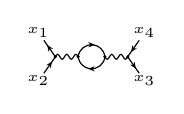
\begin{tikzpicture}[x=0.340cm, y=0.340cm, line width=0.420pt, baseline={([yshift=-0.6ex]0,0)}]
  \draw (0.500,0.000) arc[start angle=353.974, end angle=186.026, radius=0.503];
  \fill (-0.119,-0.450) -- (0.119,-0.552) -- (0.042,-0.450) -- (0.119,-0.348) -- cycle;
  \draw (-0.500,0.000) arc[start angle=173.974, end angle=6.026, radius=0.503];
  \fill (0.119,0.450) -- (-0.119,0.552) -- (-0.042,0.450) -- (-0.119,0.348) -- cycle;
  \draw plot[smooth, tension=0.7] coordinates {(-1.350,0.000) (-1.308,0.065) (-1.265,0.092) (-1.223,0.065) (-1.180,0.000) (-1.138,-0.065) (-1.095,-0.092) (-1.052,-0.065) (-1.010,0.000) (-0.968,0.065) (-0.925,0.092) (-0.883,0.065) (-0.840,0.000) (-0.798,-0.065) (-0.755,-0.092) (-0.713,-0.065) (-0.670,0.000) (-0.628,0.065) (-0.585,0.092) (-0.543,0.065) (-0.500,0.000)};
  \draw plot[smooth, tension=0.7] coordinates {(1.350,0.000) (1.308,-0.065) (1.265,-0.092) (1.223,-0.065) (1.180,0.000) (1.138,0.065) (1.095,0.092) (1.052,0.065) (1.010,0.000) (0.968,-0.065) (0.925,-0.092) (0.883,-0.065) (0.840,0.000) (0.798,0.065) (0.755,0.092) (0.712,0.065) (0.670,0.000) (0.628,-0.065) (0.585,-0.092) (0.542,-0.065) (0.500,0.000)};
  \draw (-1.350,0.000) -- (-1.780,0.614);
  \fill (-1.655,0.436) -- (-1.602,0.182) -- (-1.563,0.304) -- (-1.435,0.299) -- cycle;
  \draw (-1.350,0.000) -- (-1.780,-0.614);
  \fill (-1.475,-0.179) -- (-1.696,-0.316) -- (-1.568,-0.311) -- (-1.528,-0.433) -- cycle;
  \draw (1.350,0.000) -- (1.780,-0.614);
  \fill (1.655,-0.436) -- (1.602,-0.182) -- (1.563,-0.304) -- (1.435,-0.299) -- cycle;
  \draw (1.350,0.000) -- (1.780,0.614);
  \fill (1.475,0.179) -- (1.696,0.316) -- (1.568,0.311) -- (1.528,0.433) -- cycle;
  \fill (-1.350,0.000) circle (0.064);
  \fill (1.350,0.000) circle (0.064);
  \fill (-0.500,0.000) circle (0.064);
  \fill (0.500,0.000) circle (0.064);
  \node[font=\tiny, inner sep=0pt, anchor=305] at (-1.832,0.688) {$x_{1}$};
  \node[font=\tiny, inner sep=0pt, anchor=55] at (-1.832,-0.688) {$x_{2}$};
  \node[font=\tiny, inner sep=0pt, anchor=125] at (1.832,-0.688) {$x_{3}$};
  \node[font=\tiny, inner sep=0pt, anchor=235] at (1.832,0.688) {$x_{4}$};
\end{tikzpicture}}
\diagramgap
\mbox{$\displaystyle -\,$\,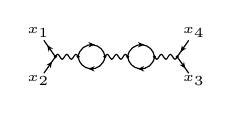
\begin{tikzpicture}[x=0.340cm, y=0.340cm, line width=0.420pt, baseline={([yshift=-0.6ex]0,0)}]
  \draw (-0.425,0.000) arc[start angle=353.974, end angle=186.026, radius=0.503];
  \fill (-1.044,-0.450) -- (-0.806,-0.552) -- (-0.883,-0.450) -- (-0.806,-0.348) -- cycle;
  \draw (-1.425,0.000) arc[start angle=173.974, end angle=6.026, radius=0.503];
  \fill (-0.806,0.450) -- (-1.044,0.552) -- (-0.967,0.450) -- (-1.044,0.348) -- cycle;
  \draw (0.425,0.000) arc[start angle=173.974, end angle=6.026, radius=0.503];
  \fill (1.044,0.450) -- (0.806,0.552) -- (0.883,0.450) -- (0.806,0.348) -- cycle;
  \draw (1.425,0.000) arc[start angle=353.974, end angle=186.026, radius=0.503];
  \fill (0.806,-0.450) -- (1.044,-0.552) -- (0.967,-0.450) -- (1.044,-0.348) -- cycle;
  \draw plot[smooth, tension=0.7] coordinates {(-2.275,0.000) (-2.232,0.065) (-2.190,0.092) (-2.148,0.065) (-2.105,0.000) (-2.062,-0.065) (-2.020,-0.092) (-1.977,-0.065) (-1.935,0.000) (-1.892,0.065) (-1.850,0.092) (-1.807,0.065) (-1.765,0.000) (-1.722,-0.065) (-1.680,-0.092) (-1.637,-0.065) (-1.595,0.000) (-1.552,0.065) (-1.510,0.092) (-1.467,0.065) (-1.425,0.000)};
  \draw plot[smooth, tension=0.7] coordinates {(2.275,0.000) (2.232,-0.065) (2.190,-0.092) (2.148,-0.065) (2.105,0.000) (2.062,0.065) (2.020,0.092) (1.978,0.065) (1.935,0.000) (1.892,-0.065) (1.850,-0.092) (1.808,-0.065) (1.765,0.000) (1.723,0.065) (1.680,0.092) (1.638,0.065) (1.595,0.000) (1.553,-0.065) (1.510,-0.092) (1.468,-0.065) (1.425,0.000)};
  \draw plot[smooth, tension=0.7] coordinates {(-0.425,0.000) (-0.382,0.065) (-0.340,0.092) (-0.297,0.065) (-0.255,0.000) (-0.212,-0.065) (-0.170,-0.092) (-0.127,-0.065) (-0.085,0.000) (-0.042,0.065) (0.000,0.092) (0.043,0.065) (0.085,0.000) (0.128,-0.065) (0.170,-0.092) (0.213,-0.065) (0.255,0.000) (0.298,0.065) (0.340,0.092) (0.383,0.065) (0.425,0.000)};
  \draw (-2.275,0.000) -- (-2.705,0.614);
  \fill (-2.580,0.436) -- (-2.527,0.182) -- (-2.488,0.304) -- (-2.360,0.299) -- cycle;
  \draw (-2.275,0.000) -- (-2.705,-0.614);
  \fill (-2.400,-0.179) -- (-2.621,-0.316) -- (-2.493,-0.311) -- (-2.453,-0.433) -- cycle;
  \draw (2.275,0.000) -- (2.705,-0.614);
  \fill (2.580,-0.436) -- (2.527,-0.182) -- (2.488,-0.304) -- (2.360,-0.299) -- cycle;
  \draw (2.275,0.000) -- (2.705,0.614);
  \fill (2.400,0.179) -- (2.621,0.316) -- (2.493,0.311) -- (2.453,0.433) -- cycle;
  \fill (-2.275,0.000) circle (0.064);
  \fill (2.275,0.000) circle (0.064);
  \fill (-1.425,0.000) circle (0.064);
  \fill (1.425,0.000) circle (0.064);
  \fill (-0.425,0.000) circle (0.064);
  \fill (0.425,0.000) circle (0.064);
  \node[font=\tiny, inner sep=0pt, anchor=305] at (-2.757,0.688) {$x_{1}$};
  \node[font=\tiny, inner sep=0pt, anchor=55] at (-2.757,-0.688) {$x_{2}$};
  \node[font=\tiny, inner sep=0pt, anchor=125] at (2.757,-0.688) {$x_{3}$};
  \node[font=\tiny, inner sep=0pt, anchor=235] at (2.757,0.688) {$x_{4}$};
\end{tikzpicture}}
